\section{Proceso Operativo SIGCSA-PO-25}

\par 
El objetivo del proceso es el de proporcionar instrucciones para la caracterización y ajustes (tomando en cuenta las instrucciones
del fabricante) de medios isotermos con el propósito de confirmar el correcto funcionamiento de
la cámara de ensayo de temperatura.\cite{po25}

\par \noindent
La caracterización es el conjunto de operaciones que determinan las diferentes
características metrológicas y especificaciones de operación de un
equipo, instrumento de medición, sistema de medición o medida
materializada. Por lo que este proceso se encarga de obtener las variables metrológicas de un equipo isotérmico, utilizando termómetros en ciertos puntos del equipo.\cite{po25}

\subsection{Alcance}
\par 
Para ser utilizados en Laboratorios Clínicos, de Ensayos, de Investigación y Bancos de Sangre, que
tengan medios isotermos de controles análogos y digitales tales como\cite{po25}:

\begin{itemize}
	\item Refrigerador de 0°C a 6°C (la conservación de sangre y derivados).
	
	\item Refrigerador de 0°C a 8°C (conservación de reactivos).
	
	\item Refrigerador de Baja Temperatura de 0°C a -35°C (conservación de reactivos y derivados
	de la sangre).
	
	\item Refrigerador de Ultra Baja Temperatura 0°C a -80°C (crio preservación de cepas y tejido
	biológico).
	
	\item Incubadoras de -10°C a 75°C (conservación de organismos vivos en un entorno que
	resulte adecuado para su crecimiento y conservación de derivados de la sangre). **
	
	\item Baño de María de temperatura ambiente a 60°C (incubación, inactivación, aglutinación y
	descongelación de derivados de la sangre).
	
	\item Baño Seco de temperatura ambiente a 60°C (incubación).
	
	\item Estufa u Horno de Secado de temperatura ambiente a 100°C (procesos de secado y
	esterilizado de recipientes de vidrio y metal).
\end{itemize}

\begin{figure}[H]
	\centering
	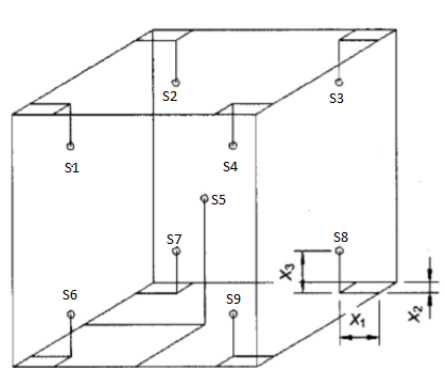
\includegraphics[width=5cm, height=4cm]{isotermo1.png}
	\caption{Medio isotermo 1, capacidad de 50L a 2100L}
\end{figure}

\begin{figure}[H]
	\centering
	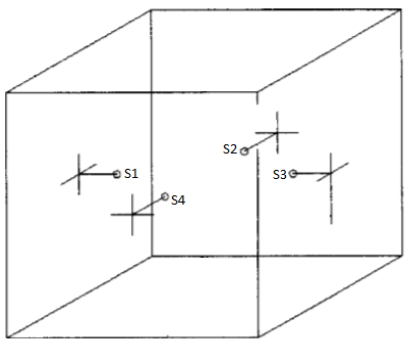
\includegraphics[width=5cm, height=4cm]{isotermo2.png}
	\caption{Medio isotermo 2, capacidad de 2L a 49L}
\end{figure}
	
\subsection{Análisis}


\par \noindent
El procedimiento se puede resumir en 4 pasos:

\begin{itemize}
	\item Preparación: Se determina las incertidumbres de los termómetros utilizados para caracterizar el medio isotermo y para validar que los termómetros se encuentran en buenas condiciones. Se documenta y se valida que las condiciones ambientales donde se encuentra el medio isotérmico son las adecuadas.
	
	\item Instalación: Si todos los parámetros del paso anterior cumplen, entonces procedemos a colocar las sondas, si el medio isotermo tiene una capacidad mayor a 49L se colocan las sondas como en la figura 2.1, en caso contrario como en la figura 2.2
	
	\item Captura de Datos: Se documenta la temperatura y humedad inicial, se captura la información que despliegan los termómetros por el tiempo estipulado en el procedimiento y una vez finalizado el tiempo nuevamente se documenta la temperatura y humedad.
	
	\item Cálculos metrológicos: Una vez capturada la información, se procede a realizar los cálculos que determinarán las características metrológicas del equipo isotérmico. 
\end{itemize}

\begin{figure}[H]
	\centering
	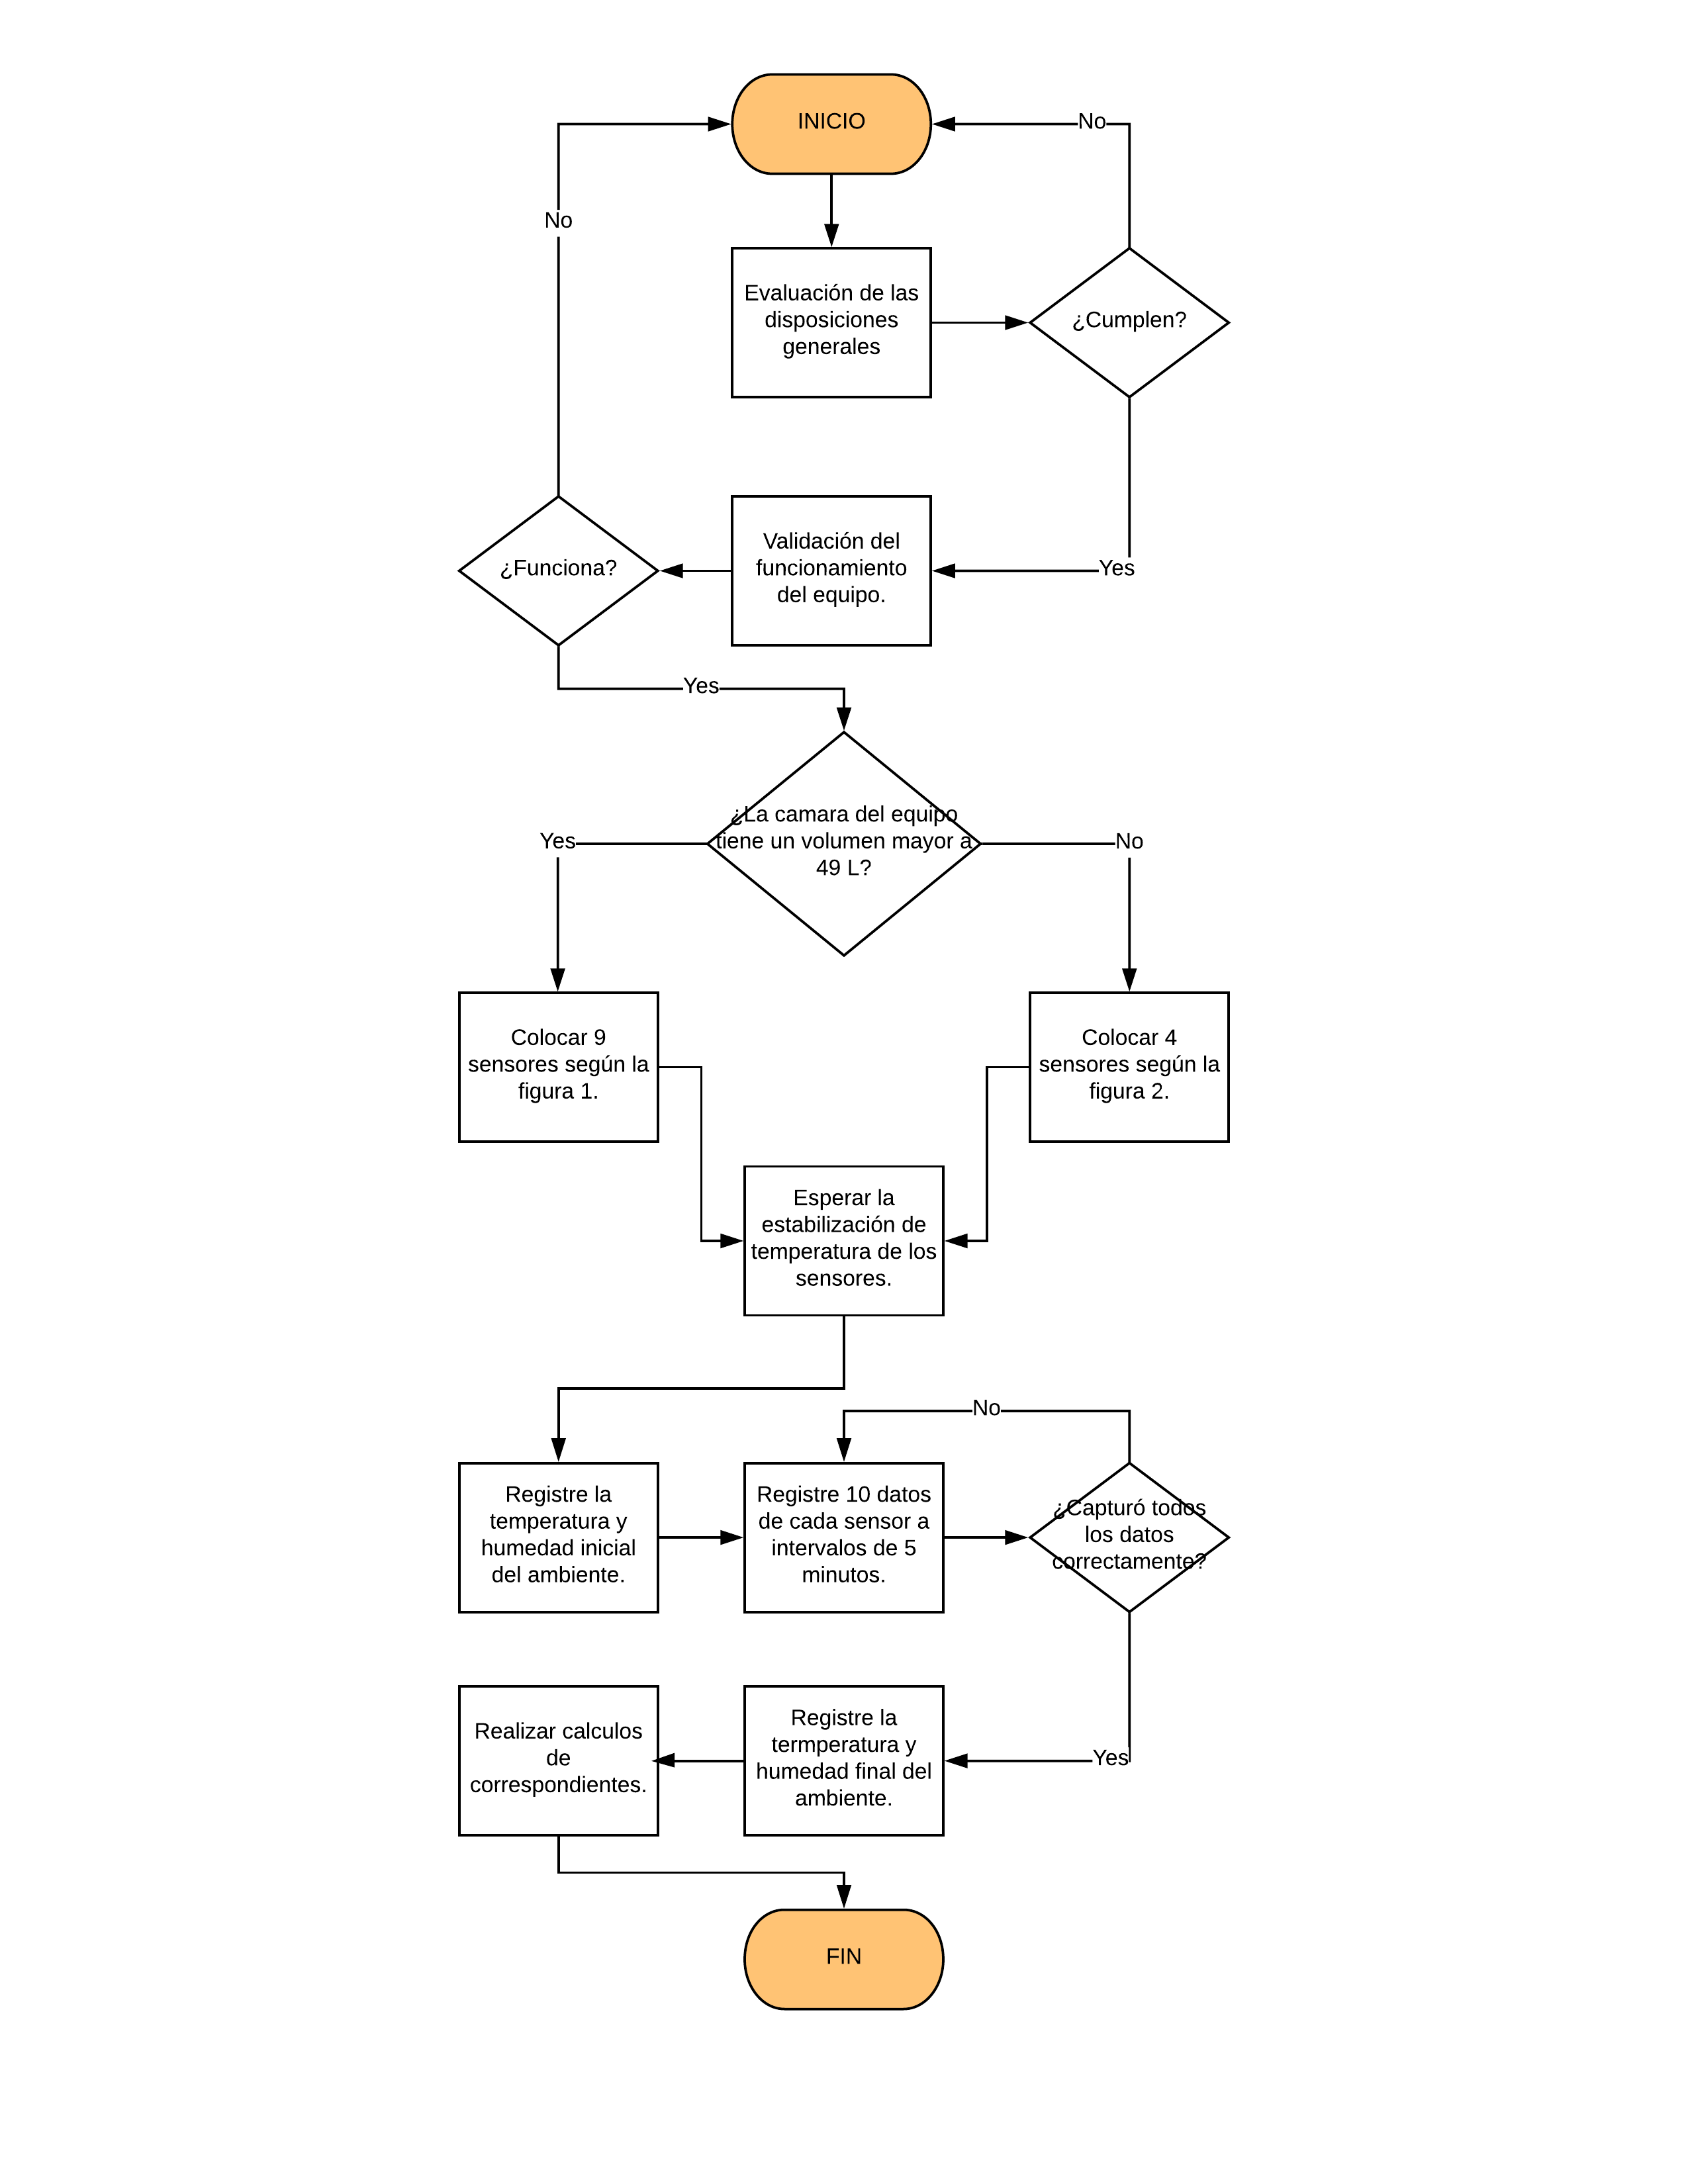
\includegraphics[width=\textwidth]{diagram1.png}
	\caption{Diagrama de flujo del proceso operativo SIGCSA-PO-25}
\end{figure}
